\begin{frame}[fragile]{Processus \texttt{Unix}}
% \begin{columns}
%   \column{0.38\linewidth}
% \begin{figure}
%     \centering
%     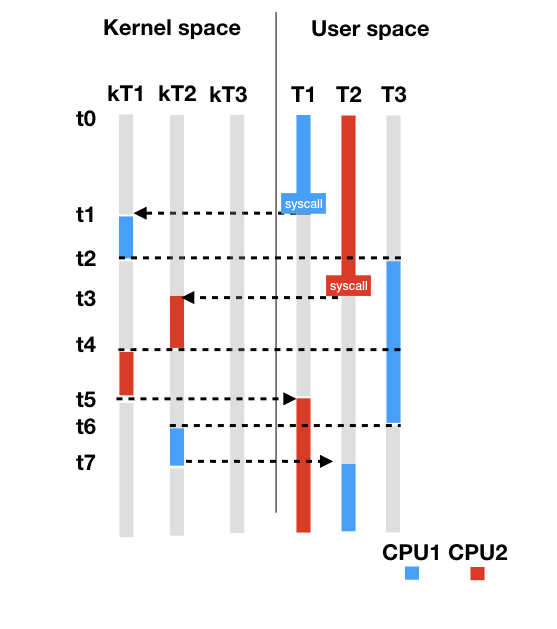
\includegraphics[width=\textwidth]{slides/images/scheduling.jpg}
% \end{figure}

% \column{0.58\linewidth}
\subtt{Un processus Unix : }
 \begin{itemize}[label=\small\ding{114}]
    \item est un programme en train de s'exécuter
    \item se compose de : 
     \begin{itemize}[label=\ding{118}]
        \item un texte de programme 
         \item un état du programme (point de contrôle courante, valeur de variables, descripteurs de fichiers ouverts etc..)
     \end{itemize}
    \item se crée avec  \begin{lstlisting}
           val fork : unit -> int 
      \end{lstlisting}
      \item le fils est une copie du père (duplique les fd par exemple)
      \item la seule différence est la valeur de sortie de \texttt{fork} : 
            \begin{itemize}[label=$-$]
                \item le fils : 0
                \item le père : l'identifiant du fils (pid)
            \end{itemize}
 \end{itemize}
% \end{columns}
\end{frame}
% \begin{frame}[fragile]{Processus Unix}
% \begin{itemize}
% \item <1->
%     \begin{lstlisting}
%         match Unix.fork () with 
%         | 0 -> (* code exécuté par le fils *)
%         | pid -> (* code exécuté par le père *)
%     \end{lstlisting}
% \item <2->
%     \begin{lstlisting}
%         val wait : unit -> int * process_status
%         val waitpid : wait_flag list -> int -> int * process_status
%         val execv : string -> string array -> 'a
%     \end{lstlisting}
%     \end{itemize}
% \end{frame}

\begin{frame}[fragile]{Boucle de lecture}
\begin{lstlisting}
    let minishell () =
       try
         while true do
           (* Lecture de l'entree standard *)
           let cmd = input_line stdin in
           match Unix.fork () with
             | 0 -> (* Processus fils *)
               let cmd = parse cmd_line in
               exec_cmd cmd;
               exit 0
             | pid_son -> (* Processus père *)
               let pid, status = Unix.wait() in
               (* Affiche le status de sortie du fils *)
                print_status "Program" status
         done
       with End_of_file -> ()

    let () = Unix.handle_unix_error minishell ()
\end{lstlisting}
\end{frame}

\subsection{Redirection et tubes}
\begin{frame}{Encore plus de fonctionnalités}
  \begin{itemize}[label=\small\ding{114}]
  \item des commandes externes (pas implémenté en OCaml (!!))
  \item des redirections (\texttt{<} \texttt{>})
  \item des tubes  (\texttt{|})
  \item les combinateurs AND et OR  (\texttt{$\&\&$} et \texttt{$||$})
  \end{itemize}
\end{frame}

\begin{frame}[fragile]{AST évolué}
    \begin{itemize}[leftmargin=-10pt]
         \item
        \begin{lstlisting}
            type cmd_kind =
                | Internal of command  (* les commandes precedentes *)
                | External of string list  (* la triche avec execvp *)
                | Cd of string
            type redirection =
                | In of string (* > *)
                | Out of string (* < *)
            type t =
                | Command of cmd_kind * redirection list
                | Pipe of t * t (* | *)
                | And of t * t  (* && *)
                | Or of t * t   (* || *)
            val execute : t -> unit
        \end{lstlisting}
    \end{itemize}
\end{frame}


\begin{frame}[fragile]{Nouvelle boucle de lecture}
\begin{lstlisting}
let minishell () =
 try
     prompt None;
     while true do
       let cmd = input_line stdin in
       try
         let cmd = Ast.parse cmd in
         let code = interprete cmd in
         prompt (Some code)
       with
       | Parser.Parsing_error err -> 
            Parser.print_error err
       | Parser.Empty_line -> ()
     done
   with End_of_file -> ()
\end{lstlisting}
\end{frame}

\begin{frame}[fragile]{Dossier courant}
 \begin{itemize}[label=$-$]
     \item pas de \texttt{fork} 
     \item \texttt{Unix.chdir : string -> unit}
     \item \texttt{Unix.getcwd : unit -> string}
 \end{itemize}
 \subtt{Implémentation:}
 \begin{lstlisting}
 let prompt = function
    | None -> Printf.printf "%s > " (Unix.getcwd ())
    | Some code -> Printf.printf "%s (%d)>" (Unix.getcwd ()) code 
 
 let rec interprete : Ast.t -> int = function
    | Ast.Command (Cd target, _) -> (
      match Unix.chdir target with 
      | exception Unix.Unix_error _ -> 1 
      | _ -> 0)
    | ...
 \end{lstlisting}
\end{frame}

\begin{frame}[fragile]{Programmes externes}
\texttt{Unix.execvp : string -> string array -> 'a} exécute le programme donné en argument en cherchant dans le \texttt{PATH}.
\begin{itemize}[label=$-$]
    \item ne retourne pas
    \item conserve l'environnement et les descripteurs ouverts
\end{itemize}
\subtt{Implémentation}
\begin{lstlisting}
let exec_cmd = function
  | Ast.Internal cmd -> Command.exec_cmd cmd
  | Ast.External (program :: _ as cmd) ->
      Unix.execvp program (Array.of_list cmd)
\end{lstlisting}
\end{frame}

\begin{frame}[fragile]{Mise à jour de \texttt{interprete}}

\begin{lstlisting}
let fork_and_wait fn =
  match Unix.fork () with
  | 0 -> fn () |> exit
  | pid_son -> (
      let _pid, status = Unix.waitpid [] pid_son in
      match status with WEXITED i -> i | WSIGNALED i -> i | WSTOPPED i -> i)

let rec interprete : Ast.t -> int = function
  | Ast.Command (Cd target, _) -> (
      match Unix.chdir target with 
      | exception Unix.Unix_error _ -> 1 
      | _ -> 0)
  | Command (cmd, redirections) ->
      fork_and_wait (fun () -> exec_cmd cmd; 0)
  | ...
\end{lstlisting}
\end{frame}